\documentclass[tikz,border=10pt]{standalone}
\usepackage{tikz}
\usetikzlibrary{arrows}
\usetikzlibrary{calc}

\begin{document}

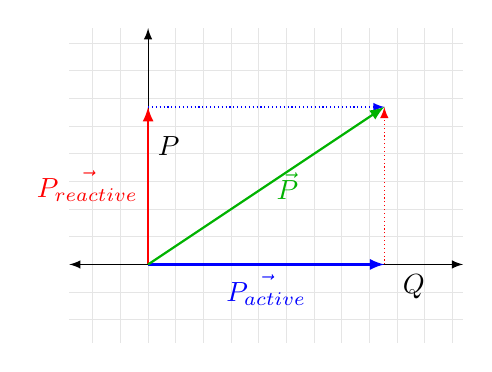
\begin{tikzpicture}[line/.style={>=latex}] 
\coordinate (V1) at (3, 0);
\coordinate (V2) at (0, 2);
\coordinate (V3) at ($(V1) + (V2)$);
\coordinate (V4) at ($1.4*(V1)$);

\draw[step=10pt, color=black!10] (-1, -1) grid (4, 3);
\draw[<->, line] (-1, 0) -- node [below, very near end] {$Q$} (4, 0);
\draw[->, line] (0, 0) -- node [right] {$P$} (0, 3);

%\draw[->, line, color=orange, thick] (0, 0) -- node [right=2pt, near end]    {$\vec{u}$} (V4);
\draw[->, line, color=blue, thick] (0, 0) -- node [below] {$\vec{P_{active}}$} (V1);

\draw[->, line, color=red, thick] (0, 0) -- node [left] {$\vec{P_{reactive}}$} (V2);
\draw[->, line, color=red, densely dotted] (V1) -- +(V2);
\draw[->, line, color=blue, densely dotted] (V2) -- +(V1);
\draw[->, line, color=green!70!black, thick] (0, 0) -- node [right] {$\vec{P}$} (V3);
\end{tikzpicture}
\end{document}